\documentclass[11pt]{article}


    \usepackage[breakable]{tcolorbox}
    \tcbset{nobeforeafter} % prevents tcolorboxes being placing in paragraphs
    \usepackage{float}
    \floatplacement{figure}{H} % forces figures to be placed at the correct location
    \usepackage{multicol}
	\usepackage[english]{babel}
    \usepackage{tabularx}
    \usepackage{subfigure}
    \usepackage{picture}
    \usepackage{amsmath}
    \usepackage{hyperref}
    \hypersetup{
    colorlinks=true,
    linkcolor=blue,
    filecolor=magenta,      
    urlcolor=cyan,
    }
    \usepackage{graphicx}    
    \usepackage{caption}
    \usepackage{adjustbox} % Used to constrain images to a maximum size 
    \usepackage{xcolor} % Allow colors to be defined
    \usepackage{enumerate} % Needed for markdown enumerations to work
    \usepackage{geometry} % Used to adjust the document margins
    \usepackage{amsmath} % Equations
    \usepackage{amssymb} % Equations
    \definecolor{urlcolor}{rgb}{0,.145,.698}
    \definecolor{linkcolor}{rgb}{.71,0.21,0.01}
    \definecolor{citecolor}{rgb}{.12,.54,.11}
    

    
    % Prevent overflowing lines due to hard-to-break entities
    \sloppy 
    % Setup hyperref package
    \hypersetup{
      breaklinks=true,  % so long urls are correctly broken across lines
      colorlinks=true,
      urlcolor=urlcolor,
      linkcolor=linkcolor,
      citecolor=citecolor,
      }
    % Slightly bigger margins than the latex defaults
    
    \geometry{verbose,tmargin=1in,bmargin=1in,lmargin=0.4in,rmargin=1in}
    \usepackage{fancyhdr}
    \pagestyle{fancy}
    \renewcommand{\footrulewidth}{1pt}
    \rhead{e11921655 Fabian Holzberger \\ e01526208 Jan Ellmenreich}
    \lhead{VU\,184.725\\ High Performance Computing}
    \cfoot{\thepage}
    \setcounter{secnumdepth}{0}
    \setlength\parindent{0pt}

    \usepackage{booktabs}

    \usepackage{listings}
    \usepackage[linesnumbered,ruled,vlined]{algorithm2e}
    \newcommand\mycommfont[1]{\footnotesize\ttfamily\textcolor{blue}{#1}}
    \SetCommentSty{mycommfont}
    \SetKwInput{KwInput}{Input}                % Set the Input
    \SetKwInput{KwOutput}{Output}              % set the Output



\title{Exercise 1 Classification}
\author{e12045110 Maria de Ronde \\ e12045110  Quentin Andre  \\ e11921655 Fabian Holzberger}
\date{\today}

\begin{document}
\graphicspath{{./figures/}}
\maketitle

%
\section{Introduction}

\subsection{Applied Algorithms}
\subsection{Performance Metrics}

\section{Amazon Reviews Dataset}
\subsection{Dataset Description}
\subsection{Pre-Processing}
\subsection{Parameter-Tuning}
\subsection{Performance-Analysis}

\section{Congressional Voting Dataset}
\subsection{Dataset Description}
\subsection{Pre-Processing}
\subsection{Parameter-Tuning}
\subsection{Performance-Analysis}


\section{Email Spam Dataset(\href{https://www.kaggle.com/nitishabharathi/email-spam-dataset}{link to dataset})}


\subsection{Dataset Description}
The task of the email spam dataset is to predict if an email is spam or not. The link above contains three datasets from which we choose two, namely the \texttt{lingSpam.csv} and \texttt{enormSpamSubset.csv} for our project, since they have no missing values and the same layout. The dataset contains 12604 emails where 43.11% are spam and 56.89% are non-spam emails.The basic structure of emails can be seen in figure \ref{tab_spam0}.

\begin{figure}[h]
  \begin{tabular}{ | c | p{15cm} | c |}
    \hline
    Index & Body & Label \\
    \hline
    100 & 
    Subject: inexpensive online medication here
 pummel wah springtail cutler bodyguard
 we ship quality medications overnight to your door !...
    & 1 \\ \hline
    6006
    &
    Subject: organizational changes
 we are pleased to announce the following organizational changes :
 enron global assets and services
 in order to increase senior management focus on our international businesses... 
    & 0 \\
    \hline
    \end{tabular}
    \caption{Structure of the Email-Spam Dataset}
    \label{tab_spam0}
  \end{figure}
Every email has a binary target-label assigned, such that a 0 marks non-spam and a 1 marks spam emails. In figure \ref{fig_fig0} the distribution of the characters per email is shown. We see that most emails have a lenght in the range of 100 to 10.000 characters.

\begin{figure}
\begin{minipage}[t]{0.3\textwidth}
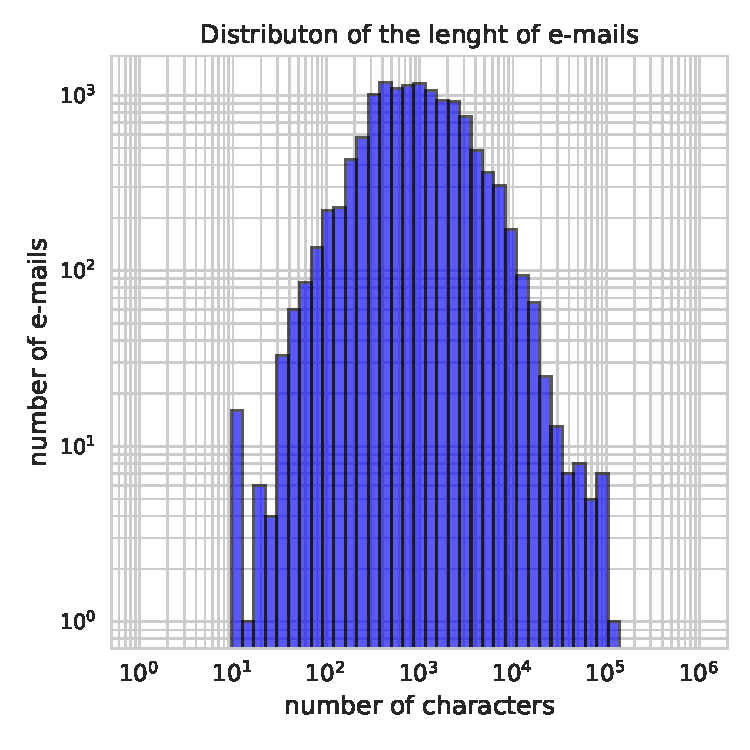
\includegraphics[width=1\linewidth]{email_spam/char_count.pdf}
\end{minipage}
\begin{minipage}[t]{0.3\textwidth}
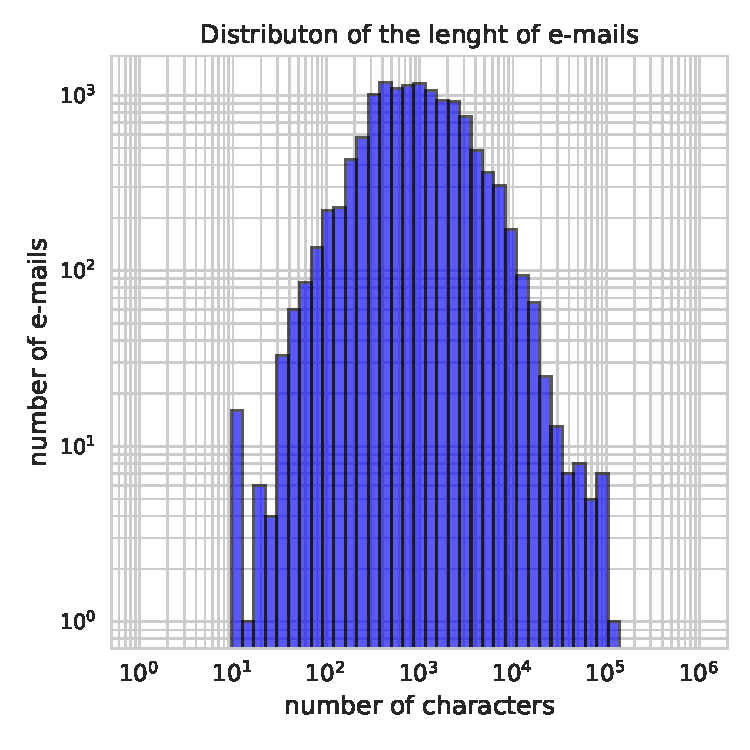
\includegraphics[width=1\linewidth]{email_spam/char_count.pdf}
\end{minipage}
\begin{minipage}[t]{0.3\textwidth}
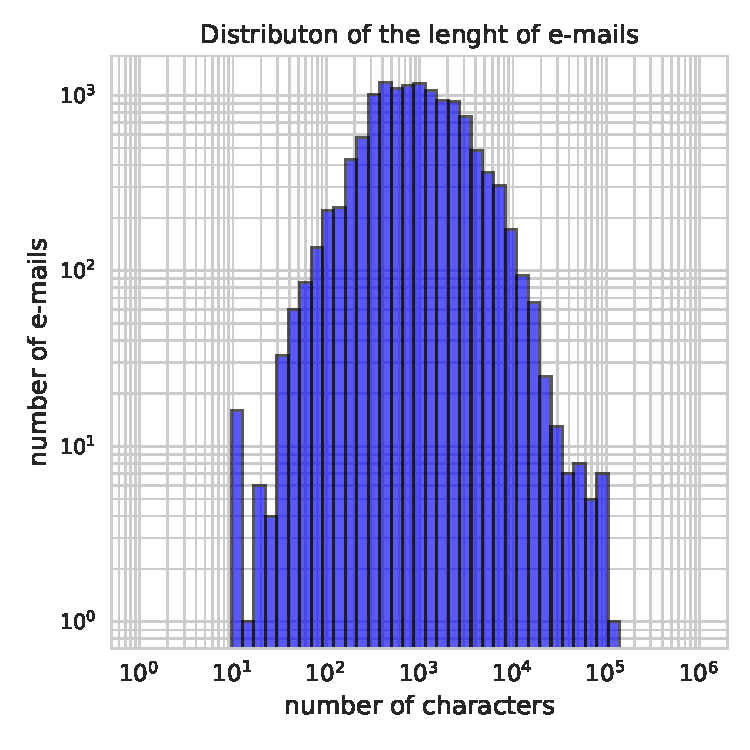
\includegraphics[width=1\linewidth]{email_spam/char_count.pdf}
\end{minipage}
   \caption{left: Distribution of e-mail lenghts }
\label{fig_fig0}
\end{figure}

We apply the Bag of Words feature extractor to each email. The algorithm converts every email to a vector $v\in\mathbb{N^+}^N$ of intergers. First we create a list of all words and count their occurences in all emails. Then we take the $N$ most common words and count the occurences of the most common words in every email ti get $v$. Before applying the Bag of word extractor we pre-process emails by the following steps:



\subsection{Pre-Processing}
\subsection{Parameter-Tuning}
\subsection{Performance-Analysis}


\section{Bridges Dataset(\href{https://archive.ics.uci.edu/ml/datasets/Pittsburgh+Bridges}{link to dataset})}
\subsection{Dataset Description}
\subsection{Pre-Processing}
\subsection{Parameter-Tuning}
\subsection{Performance-Analysis}

\section{Conclusion}

%Bibliography
\newpage
\bibliographystyle{plain}
\bibliography{Biblothek}

\end{document}
